\documentclass[12pt]{article}
\usepackage[english, russian]{babel}
\usepackage[TS1, T2A]{fontenc}
\usepackage[utf8]{inputenc}
\usepackage{hyperref}
\usepackage{pscyr}
\usepackage{graphicx}
\usepackage{enumitem,kantlipsum}
\graphicspath{{pictures/}}
\DeclareGraphicsExtensions{.jpg}
\usepackage[left=2cm,right=2cm, top=1cm,bottom=1.5cm,bindingoffset=0cm]{geometry}
\begin{document}
\pagestyle{empty}
\begin{center}
\normalsize
\textbf{Федеральное государственное автономное образовательное учреждение высшего образования}

\small
\medskip 
\textbf{САНКТ-ПЕТЕРБУРГСКИЙ НАЦИОНАЛЬНЫЙ ИССЛЕДОВАТЕЛЬСКИЙ  УНИВЕРСИТЕТ ИНФОРМАЦИОННЫХ ТЕХНОЛОГИЙ, МЕХАНИКИ И ОПТИКИ}

\medskip 
\textbf{ФАКУЛЬТЕТ ПРОГРАММНОЙ ИНЖЕНЕРИИ И КОМПЬЮТЕРНОЙ ТЕХНИКИ}
\end{center}
\bigskip\bigskip\bigskip\bigskip\bigskip\bigskip\bigskip\bigskip\bigskip\bigskip\bigskip\bigskip
\begin{center}
\par\medskip\par\smallskip
\Large
 
\par\smallskip
\textbf{ОТЧЕТ} 

\textbf{ПО ЛАБОРАТОРНОЙ РАБОТЕ №2}

\large
\par\bigskip
\textbf{«Аппаратное обеспечение и другие особенности систем.} 

\textbf{Оптимизация алгоритма для определенных архитектур»}
\par\bigskip\par\bigskip\par\bigskip\par\bigskip\par\bigskip\par\bigskip
\par\bigskip\par\bigskip\par\bigskip\par\bigskip\par\bigskip\par\bigskip
\par\bigskip\par\bigskip\par\bigskip\par\bigskip\par\bigskip\par\bigskip
\end{center}
\begin{center}
\begin{tabular}{lllll}
Проверил:	 	  							& \hspace{80pt}	&	Выполнил:								&\\
Сентерев Ю.А.	 \_\_\_\_\_\_\_\_\_\_\_\_\_\_		&			&	Студент группы P3255					&\\
«\_\_\_\_\_\_» 	\_\_\_\_\_\_\_\_\_\_\_\_\_\_ 201\_г.	& 			&	Федюкович С. А. \_\_\_\_\_\_\_\_\_\_\_\_\_\_	&\\
										&			&										&\\
Оценка\hspace{12pt}\_\_\_\_\_\_\_\_\_\_\_\_\_\_	&			&										&\\
\end{tabular}
\par\bigskip\par\bigskip\par\bigskip
                                                  
\par\bigskip \par\bigskip
\end{center}
\par\bigskip\par\bigskip\par\bigskip\par\bigskip\par\bigskip\par\bigskip\par\bigskip\par\bigskip
\begin{center}
Санкт-Петербург
\par\bigskip
2018
\end{center}
\newpage
\pagestyle{plain}
\setcounter{page}{1}
	\section*{Цель работы}
	Самосмоятельно разобрать и изучить понятия аппаратного обеспечения и его компонентов. Также познакомиться с оптимизацией алгоритмов на определенных архитектурах. 

	\section*{Ход работы}
	\subsection*{Аппаратное обеспечение}
	Аппаратное обеспечение (АО) представляет собой совокупность технических средств. Обычно это электронные и механические устройства. Они позволяют обеспечить как нормальное функционирование каких-либо систем, так и расширяющих их основные функции. В первом случае это могут быть компьютеры, сети передачи данных.
	
	\begin{center}
		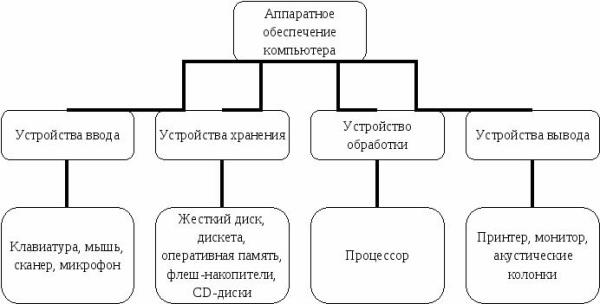
\includegraphics{1}
	\end{center}	
	
	В современном обществе основным техническим средством технологии переработки информации служит персональный компьютер, который существенно повлиял как на концепцию построения и использование технологических процессоров, так и на качество результатной информации. Компьютерная технология --- это информационный процесс, в результате которого создается информационный продукт на базе компьютерной обработки данных.\\
		
	\subsection*{Основные комплектующие АО}
	\begin{enumerate}[wide, labelwidth=!, labelindent=0pt]
		\item Процессор, CPU ---  устройство, выполняющее команды компьютерной системы. В современных компьютерах, как правило, он является многоядерным, т.е. имеет в своем составе от 2 до 32 ядер (копий) процессора, параллельно работающих на общей памяти, либо гибридным, состоящим из центрального и графического процессоров. Производительность каждого ядра – 3 – 3.2 GHz --- время выполнения им одной самой простой машинной команды. Однако есть и другие важные факторы, определяющие общую производительность системы, --- тактовая частота памяти и системной шины. Фактически итоговую производительность системы можно оценить по самой медленной из этих частей системы (обычно это системная шина). Эти характеристики необходимо принимать во внимание при выборе и покупке компьютера.
		\item Материнская плата --- базовый элемент архитектуры, представляет собой многоуровневую плату с предустановленным набором микросхем системной логики, служит для объединения комплектующих в единую систему (компьютер).
		\item Оперативная (основная) память, или просто память– устройство, хранящее обрабатываемые данные. Объем памяти – 1 – 16 гигабайт и более; меньший объем памяти использовать не рекомендуется, так как это может привести к значительному замедлению системы. Тактовая частота памяти – 667 MHz – 1.5 GHz.
		\item Жёсткий диск (HDD) --- энергонезависимое запоминающее устройство, назначение которого длительное хранение данных. Информация сохраняется на жестких носителях (дисках из специальных сплавов) имеющих ферромагнитное покрытие (двуокись хрома).
		\item Блок питания ---  основной источник энергии, от которого зависит стабильная работа всей системы. Задача БП преобразовывать переменное сетевое напряжение в пониженное постоянное: 3.3 и 5В – для питания микросхем; 12В – для снабжения энергией остальных комплектующих.
		\item Устройства ввода-вывода --- отдельный вид устройств предназначенный для взаимодействия с АО. Используются для внесения, редактирования и удаления данных.
		\item Системная шина --- устройство, к которому подсоединены все модули компьютера и через которое они обмениваются сигналами, например, о прерываниях. Тактовая частота шины – 1 – 1.5 GHz (это и есть фактически некая суммарная производительность системы). Обычно используется шина типа PCI (Peripheral Component Interconnect). К ней могут быть подсоединены процессор, память, диски, принтер, модем и другие внешние устройства.
		\item Порты --- устройства с разъемами для подключения к компьютеру внешних устройств. Каждый порт имеет свой контроллер (и, соответственно, свой драйвер). Чаще всего используется порт USB (Universal Serial Bus),с характерным плоским разъемом. Порты COM (communication ports) --- порты для подключения различных коммуникационных устройств, например, модемов– устройств для выхода в Интернет и передачи информации по аналоговой или цифровой телефонной линии. Порт LPT(от line printer), или параллельный порт --- это ныне уже устаревший вид порта для подключения принтера или сканера, с толстым в сечении кабелем и большим разъемом. Все новые модели принтеров и сканеров работают через USB-порты. SCSI (Small Computer System Interface) --- интерфейс, адаптеры и порты для подключения широкого спектра внешних устройств – жестких дисков, CD-ROM / DVD-ROM, сканеров и др. Порт VGA (Video Graphic Adapter) --- используется для подключения монитора, управляемого графическим контроллером. IEEE 1394 (FireWire) --- порты для подключения цифровых видеокамер или фотоаппаратов. HDMI (High Definition Multimedia Interface) --- интерфейс и порт. позволяющий подключить к компьютеру телевизор или другое видеооборудование, обеспечивающее наилучшее качество воспроизведения. Bluetooth-устройства для беспроводного подключения (с помощью радиосвязи) к компьютеру мобильных телефонов, органайзеров, а также наушников, плейеров и многих других полезных устройств. нфракрасный порт (IrDA)– порт для подключения ноутбука к мобильному телефону (или двух ноутбуков друг к другу) через инфракрасную связь.
	\end{enumerate}	
	
	\subsection*{Серверное аппаратное обеспечение}
	Стоит отметить, что к аппаратному обеспечению относятся также серверы. Они представляют собой узкоспециализированные решения. Для них свойственно встроенное программное обеспечение, оно определяется специализацией и возможными предоставляемыми услугами. Аппаратное обеспечение данного вида отличается простотой и надежностью эксплуатации. Серверы потребляют намного меньше электроэнергии и в ряде случаев оказываются дешевле по стоимости. Но здесь следует отметить и некоторый минус. Их гибкость несколько меньше, а также такое обеспечение иногда ограничивается в ресурсах.
	
	Главной особенностью является то, что сервер в первую очередь является программой или программным модулем. Без этого исключается вероятность существования аппаратного обеспечения. Важно помнить, что на одной единице АО может единовременно производиться произвольное количество серверов. Исключением являются только те, которые конфликтуют между собой по ресурсам и их количеству. Это связано с тем, что будет происходить деление.
	
	Приводить в действие услуги серверов возможно на рабочей станции. Это необходимо для их функционирования на фоне разделения ресурсов компьютера с программными продуктами, которые запускаются пользователем. Такой принцип получил название «невыделенного». В противном случае компьютером выполняются только сервисные функции. При этом на рабочей станции уже может быть несколько серверов. Обычно им является терминальный и удаленного доступа к файловой системе и системе печати.
	
	\subsection*{Оптимизация на определенных архитектурах}
	Оптимизация --- это процесс преобразования фрагмента кода в другой фрагмент, который функционально эквивалентен исходному, с целью улучшения одной или нескольких его характеристик, из которых наиболее важными являются скорость и размер кода.
	
	Основной задачей при проектировании, разработке или модернизации сложных программных систем, как и любых других сложных объектов, для разработки которых привлекаются ресурсы разного характера и объема, является создание соответствующего объекта с заданным уровнем качества в условиях ограниченности ресурсов. 
	
	Для сложных информационных систем, используемых в критических областях (технологические процессы, управление движением, финансовые операции) возникает задача построения такой архитектуры программного обеспечения (ПО), чтобы оно обладало заданной надежностью и требовало на реализацию минимальных трудозатрат. 
	
	Компоненты архитектуры программного обеспечения могут быть реализованы с использованием программной избыточности. Если вводится программная избыточность, то ее можно реализовать методом мультиверсионного программирования (NVP – N-version programming) или блока восстановления (RB – recovery block). 
	
	Программный компонент или каждая его версия, в случае применения программной избыточности, могут быть доведены до определенного уровня надежности (вероятности сбоя) путем тестирования. С помощью статистических моделей надежности или экспертных оценок, могут быть определены варианты возможного уровня надежности компонента (или его версии) и соответствующих трудозатрат на достижение этого уровня надежности. 
	
	Таким образом, возникает задача оптимизации характеристик определенных компонентов архитектуры ПО. Задача сводится к поиску максимума функции коэффициента готовности проектируемой системы и минимума функции ресурсов, затрачиваемые на разработку или модификацию программной системы.
	
	\section*{Вывод}
	В ходе работы я изучил достаточно источников, кратко изложив суть аппаратного обеспечения и оптимизации в работе. Цель достигнута
	
	\newpage
	\section*{Список источников}
\begin{enumerate}[wide, labelwidth=!, labelindent=0pt]
\item \href{https://www.elektro-expo.ru/ru/ui/17028/}{www.elektro-expo.ru/ru/ui/17028} --- Аппаратное обеспечение: особенности устройств, комплектующих 
\item \href{https://www.2hpc.ru/аппаратное-обеспечение/}{www.2hpc.ru/аппаратное-обеспечение} --- Аппаратное обеспечение (hardware, «железо»)
\item \href{https://www.helpiks.org/6-54866.html}{www.helpiks.org/6-54866.html} --- Аппаратное обеспечение
\item \href{http://csaa.ru/apparatnoe-obespechenie-kompjutera/}{www.csaa.ru/apparatnoe-obespechenie-kompjutera} --- Аппаратное обеспечение компьютера
\item \href{http://csaa.ru/arhitektura-kompjuternoj-sistemy/}{www.csaa.ru/arhitektura-kompjuternoj-sistemy} --- Архитектура компьютерной системы
\item \href{https://habr.com/company/intel/blog/338870/}{www.abr.com/company/intel/blog/338870} --- Оптимизация TensorFlow на современных архитектурах Intel
\item \href{http://4by4.ru/services/ITArchitecture}{www.4by4.ru/services/ITArchitecture} --- Оптимизация архитектуры приложений банка
\item \href{https://habr.com/company/enterra/blog/250199/}{www.habr.com/company/enterra/blog/250199} --- Что каждый программист должен знать про оптимизации компилятора
\item Вестник воронежского государственного университета. Cерия: Cистемный анализ и информационные технологии  --- Оптимизация программной архитектуры на основе генетического алгоритма с аллелями в шкале порядка
\item Логистические системы в глобальной экономике --- Оптимизация программной архитектуры логистических информационных систем
\end{enumerate} 
\end{document}